\chapter{Theoretical Foundations}
\label{chap:theory}

This chapter introduces the mathematical background needed for the rest of the thesis.
Section~\ref{sec:mdp} reviews Markov Decision Processes.
Section~\ref{sec:pomdp} introduces Partially Observable MDPs.
Section~\ref{sec:comp} discusses the computational challenges of exact POMDP solving.
Section~\ref{sec:pwlc} explains the piecewise linear and convex structure of the value function, which is central to understanding both exact and approximate algorithms.


\section{Markov Decision Processes}
\label{sec:mdp}

A Markov Decision Process (MDP) models sequential decision-making in fully observable, stochastic environments \cite{algorithmsSequentialDecisionMaking}.
Formally, an MDP is defined by a tuple $\langle S, A, T, R, \gamma \rangle$ where:
\begin{itemize}
  \item $S$ is a finite set of states,
  \item $A$ is a finite set of actions,
  \item $T: S \times A \times S \rightarrow [0,1]$ is the transition function, where $T(s, a, s')$ gives the probability of moving to state $s'$ after taking action $a$ in state $s$,
  \item $R: S \times A \rightarrow \mathbb{R}$ is the reward function, and
  \item $\gamma \in [0,1)$ is a discount factor.
\end{itemize}

The Markov property holds: the next state depends only on the current state and action, not on the history.
The agent's goal is to find a policy $\pi: S \rightarrow A$ that maximizes the expected discounted cumulative reward:
\begin{equation}
  V^\pi(s) = \mathbb{E}\!\left[\sum_{t=0}^{\infty} \gamma^t R(s_t, a_t) \;\middle|\; s_0 = s,\; a_t = \pi(s_t)\right].
\end{equation}

The optimal value function $V^*$ satisfies the Bellman equation:
\begin{equation}
  V^*(s) = \max_{a \in A} \left[ R(s, a) + \gamma \sum_{s' \in S} T(s, a, s')\, V^*(s') \right].
\end{equation}

This can be solved by value iteration, which applies the Bellman backup operator repeatedly until convergence.
MDPs are well understood and scalable to large state spaces \cite{mdpBasedRecommenderSystem}.
They serve as the foundation for POMDPs, which relax the assumption that the state is directly observed.


\section{Partially Observable Markov Decision Processes}
\label{sec:pomdp}

A POMDP extends the MDP framework to settings where the agent cannot observe the true state directly \cite{astrom1965optimal,kaelblingPlanningActingPartially1998}.
An observation model is added: after taking an action, the agent receives an observation that depends on the resulting state.

Formally, a POMDP is a tuple $\langle S, A, T, R, \Omega, O, \gamma \rangle$ where:
\begin{itemize}
  \item $S$, $A$, $T$, $R$, $\gamma$ are as in the MDP,
  \item $\Omega$ is a finite set of observations, and
  \item $O: S \times A \times \Omega \rightarrow [0,1]$ is the observation function, where $O(s', a, o)$ gives the probability of observing $o$ after arriving in state $s'$ by taking action $a$.
\end{itemize}

Since the agent does not observe the state, it must reason about which states are possible given its history of actions and observations.
This is captured by the belief state $b \in \Delta(S)$, a probability distribution over $S$ \cite{pomdpIntroNotes}.
After taking action $a$ and observing $o$, the belief is updated using Bayes' rule:
\begin{equation}
  b'(s') = \frac{O(s', a, o) \sum_{s \in S} T(s, a, s')\, b(s)}{P(o \mid b, a)},
\end{equation}
where the normalizing constant is $P(o \mid b, a) = \sum_{s' \in S} O(s', a, o) \sum_{s \in S} T(s, a, s')\, b(s)$.

The belief state is a sufficient statistic for the history: the optimal policy depends only on $b$, not on the full sequence of past states and observations \cite{smallwood1973optimal}.
This makes POMDPs tractable in principle, because the problem reduces to an MDP over the continuous belief space $\Delta(S)$.

POMDPs have been applied to a wide range of problems \cite{pomdpsMixedObservabilityRoboticTasks}.
In robotic navigation, the agent does not always know where it is, and the observation model describes which sensor readings are likely in each location \cite{kurniawatiPartiallyObservableMarkov2022}.
In manipulation tasks, the POMDP models uncertainty about object poses and contact outcomes \cite{pajarinenPOMDPPlanningObject2023}.


\section{Computational Challenges}
\label{sec:comp}

Solving a POMDP exactly is much harder than solving an MDP.
The belief space is a continuous simplex $\Delta(S)$, so the value function is defined over an uncountably infinite domain.
Exact value iteration requires computing a backup over all possible next beliefs, which is expensive.

The key result, due to Smallwood and Sondik \cite{smallwood1973optimal}, is that the value function after any finite number of steps is piecewise linear and convex (PWLC).
Specifically, it can be written as:
\begin{equation}
  V(b) = \max_{\alpha \in \Gamma} \sum_{s \in S} \alpha(s)\, b(s) = \max_{\alpha \in \Gamma}\; \alpha \cdot b,
\end{equation}
where $\Gamma$ is a finite set of vectors $\alpha \in \mathbb{R}^{|S|}$, each called an alpha vector.
This makes exact computation feasible in principle: each backup step produces a new finite set of alpha vectors.

However, the number of alpha vectors can grow exponentially.
At each backup step, the number of candidate alpha vectors per action is $|\Gamma|^{|\Omega|}$, since for each observation we select one vector from the current set \cite{cassandra1994acting}.
Even with pruning, the set $\Gamma$ can become very large for problems with many actions or observations.
This is the core computational challenge: exact POMDP solving does not scale gracefully.

The problem is also known to be PSPACE-complete in general \cite{cassandra1994acting}.
This means we cannot expect a polynomial-time algorithm.
For small problems, exact methods work well.
For larger ones, approximate algorithms are necessary \cite{hauskrechtValuefunctionApproximationsPartially2000}.


\section{The Geometry of the Value Function}
\label{sec:pwlc}

Understanding the geometric structure of the value function helps explain both how exact algorithms work and why they become expensive.
This section looks at that structure more carefully.


\subsection{The PWLC Property}

The belief space for an $|S|$-state POMDP is the $(|S|-1)$-dimensional simplex:
\begin{equation}
  \Delta(S) = \left\{ b \in \mathbb{R}^{|S|} \;\middle|\; b(s) \geq 0 \text{ for all } s,\; \sum_{s} b(s) = 1 \right\}.
\end{equation}
Each alpha vector $\alpha \in \Gamma$ defines a hyperplane over this simplex.
The value function is the upper envelope of these hyperplanes:
\begin{equation}
  V(b) = \max_{\alpha \in \Gamma}\; \alpha \cdot b.
\end{equation}
This upper envelope is by definition piecewise linear and convex.
Figure~\ref{fig:pwlc} illustrates this for a two-state POMDP, where the belief space collapses to the unit interval $[0,1]$.

\begin{figure}[htbp]
  \centering
  % TikZ figure: PWLC value function for a two-state POMDP
% Illustrates how the value function is piecewise linear and convex
% over the one-dimensional belief space b = Pr(s1)

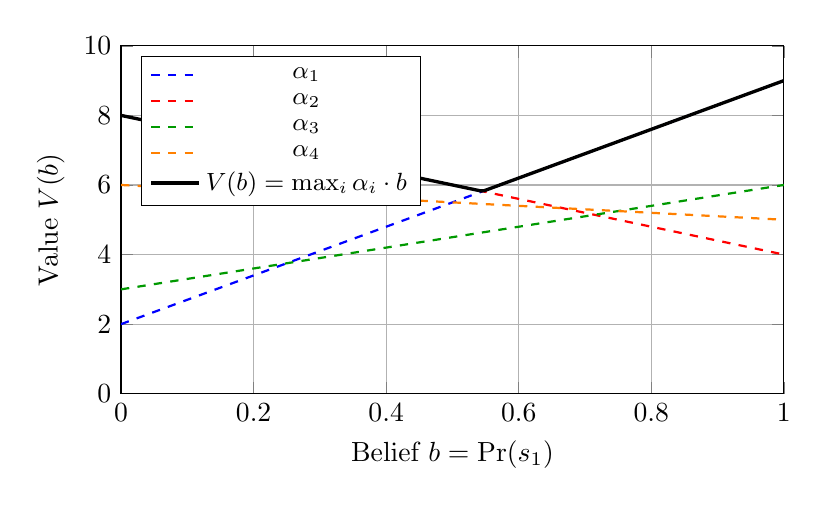
\begin{tikzpicture}[scale=1.0]
  \begin{axis}[
    width=10cm,
    height=6cm,
    xlabel={Belief $b = \Pr(s_1)$},
    ylabel={Value $V(b)$},
    xmin=0, xmax=1,
    ymin=0, ymax=10,
    xtick={0, 0.2, 0.4, 0.6, 0.8, 1.0},
    ytick={0, 2, 4, 6, 8, 10},
    grid=both,
    grid style={line width=0.2pt, draw=gray!30},
    major grid style={line width=0.4pt, draw=gray!60},
    legend pos=north west,
    legend style={font=\small},
  ]

    % Individual alpha vectors (linear functions of b)
    \addplot[blue,   dashed, thick, domain=0:1] {2 + 7*x}   node[right, pos=1] {};
    \addplot[red,    dashed, thick, domain=0:1] {8 - 4*x}   node[right, pos=1] {};
    \addplot[green!60!black, dashed, thick, domain=0:1] {3 + 3*x} node[right, pos=1] {};
    \addplot[orange, dashed, thick, domain=0:1] {6 - 1*x}   node[right, pos=1] {};

    % The PWLC envelope (upper envelope = value function)
    \addplot[black, very thick, domain=0:1, samples=200] {max(max(2+7*x, 8-4*x), max(3+3*x, 6-1*x))};

    \addlegendentry{$\alpha_1$}
    \addlegendentry{$\alpha_2$}
    \addlegendentry{$\alpha_3$}
    \addlegendentry{$\alpha_4$}
    \addlegendentry{$V(b) = \max_i \alpha_i \cdot b$}

  \end{axis}
\end{tikzpicture}

  \caption{
    The PWLC value function for a two-state POMDP.
    Each dashed line corresponds to one alpha vector.
    The solid line is the value function, which is the upper envelope of all alpha vectors.
    Each alpha vector is optimal over the region of the belief space where it is highest.
  }
  \label{fig:pwlc}
\end{figure}

This representation is compact: instead of storing a value for every belief point (which is impossible since the space is infinite), we store a finite list of vectors.
Each vector encodes a linear policy over part of the belief space.


\subsection{Alpha Vectors and Belief Simplex Partitioning}

Each alpha vector $\alpha_i \in \Gamma$ is associated with an action $a_i$.
At any belief $b$, the agent should take the action corresponding to the alpha vector that achieves the maximum:
\begin{equation}
  \pi^*(b) = a_i \quad \text{where } i = \arg\max_{j} \alpha_j \cdot b.
\end{equation}
This partitions the belief simplex into regions: each region consists of all beliefs where one particular alpha vector dominates.
Within each region, the optimal action is the same.

Figure~\ref{fig:simplex} shows this partition for a three-state POMDP.
The simplex has three vertices, each corresponding to certainty about one state.
The dashed lines divide the simplex into regions, and each region is labelled with the dominant alpha vector.

\begin{figure}[htbp]
  \centering
  % TikZ figure: Belief simplex partition for a three-state POMDP
% Each region corresponds to the belief points where one alpha vector dominates

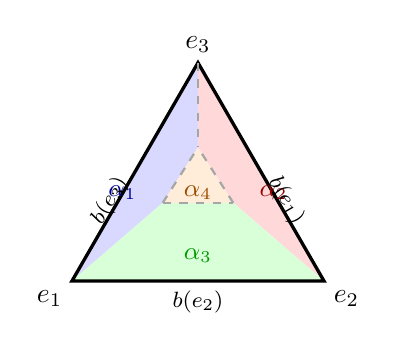
\begin{tikzpicture}[scale=3.2]

  % Define the three vertices of the simplex
  \coordinate (v0) at (0,   0);      % b = (1,0,0): all mass on s0
  \coordinate (v1) at (1,   0);      % b = (0,1,0): all mass on s1
  \coordinate (v2) at (0.5, 0.866);  % b = (0,0,1): all mass on s2

  % Partition boundaries (approximate dividing lines inside simplex)
  \coordinate (c1) at (0.36, 0.31);
  \coordinate (c2) at (0.64, 0.31);
  \coordinate (c3) at (0.50, 0.53);

  % Fill the three regions with light colors
  \fill[blue!15]   (v0) -- (c1) -- (c3) -- (v2) -- cycle;
  \fill[red!15]    (v1) -- (c2) -- (c3) -- (v2) -- cycle;
  \fill[green!15]  (v0) -- (c1) -- (c2) -- (v1) -- cycle;
  \fill[orange!15] (c1) -- (c2) -- (c3) -- cycle;

  % Draw the simplex outline
  \draw[very thick] (v0) -- (v1) -- (v2) -- cycle;

  % Draw partition boundaries
  \draw[thick, dashed, gray!70] (v2) -- (c3);
  \draw[thick, dashed, gray!70] (c1) -- (c3);
  \draw[thick, dashed, gray!70] (c2) -- (c3);
  \draw[thick, dashed, gray!70] (c1) -- (c2);

  % Label vertices
  \node[below left]  at (v0) {$e_1$};
  \node[below right] at (v1) {$e_2$};
  \node[above]       at (v2) {$e_3$};

  % Region labels
  \node[blue!60!black,   font=\small] at (0.20, 0.35) {$\alpha_1$};
  \node[red!60!black,    font=\small] at (0.80, 0.35) {$\alpha_2$};
  \node[green!60!black,  font=\small] at (0.50, 0.10) {$\alpha_3$};
  \node[orange!60!black, font=\small] at (0.50, 0.35) {$\alpha_4$};

  % Axis labels along edges (matching vertex notation e_1, e_2, e_3)
  \node[below, font=\footnotesize] at (0.5, 0) {$b(e_2)$};
  \node[left,  font=\footnotesize, rotate=60] at (0.22, 0.44) {$b(e_3)$};
  \node[right, font=\footnotesize, rotate=-60] at (0.78, 0.44) {$b(e_1)$};

\end{tikzpicture}

  \caption{
    Partitioning of the three-state belief simplex by alpha vectors.
    Each shaded region corresponds to beliefs where one alpha vector achieves the maximum value.
    The dashed lines mark the boundaries between regions.
    Vertices $e_1$, $e_2$, $e_3$ represent degenerate beliefs concentrated on one state.
  }
  \label{fig:simplex}
\end{figure}

The number of regions can be large.
As the planning horizon grows, more alpha vectors are added, and the partition becomes finer.
This is why the alpha vector set is the central data structure in POMDP solvers \cite{shaniSurveyPointbasedPOMDP2013}.


\subsection{Value Iteration via Back-Projection}

The exact backup operator computes a new set of alpha vectors from the current set.
The idea is that, for each action and each possible observation, we can compute how the current alpha vectors transform under the POMDP dynamics.
The new alpha vectors are formed by combining these back-projected pieces \cite{smallwood1973optimal,hauskrechtValuefunctionApproximationsPartially2000}.

For a given action $a$ and observation $o$, the back-projected vector $\alpha_{a,o,i}$ is:
\begin{equation}
  \alpha_{a,o,i}(s) = \sum_{s' \in S} O(s', a, o)\, T(s, a, s')\, \alpha_i(s'),
\end{equation}
where $\alpha_i$ is a vector from the previous iteration.
The full backup for action $a$ then selects the best combination across observations:
\begin{equation}
  \alpha_a(s) = R(s, a) + \gamma \sum_{o \in \Omega} \max_{\alpha_i \in \Gamma}\; \alpha_{a,o,i}(s).
\end{equation}
The new set $\Gamma'$ is formed by taking the union over all actions and then pruning dominated vectors.

This process is exact but expensive.
The number of candidate vectors per action is $|\Gamma|^{|\Omega|}$ before pruning.
Even after pruning, $|\Gamma|$ can still grow very quickly \cite{incrementalPruningNotes}.


\subsection{Why Approximate Algorithms Are Necessary}

The exponential growth of alpha vectors makes exact methods impractical for most real problems.
Consider a POMDP with 25 states, 4 actions, and 5 observations.
After just a few iterations, the number of alpha vectors can reach thousands.
Memory and computation both become bottlenecks.

Point-based methods address this by restricting updates to a finite set of sampled belief points \cite{pineauPointbasedValueIteration,spaanPerseusRandomizedPointbased2005}.
Instead of covering the entire simplex, they compute alpha vectors that are useful near the sampled beliefs.
This trades global optimality for tractability.

HSVI and related methods use heuristic search to focus sampling on reachable and informative beliefs \cite{smithHeuristicSearchValue}.
Multi-resolution approaches decompose the problem to handle large state spaces \cite{zhengMultiResolutionPOMDPPlanning2022}.
The QMDP heuristic collapses the problem to a simpler MDP as a fast approximation \cite{zhangModelApproximationScheme1997}.

All of these methods are grounded in the PWLC representation.
Understanding the geometry of the value function is therefore essential for understanding what each algorithm does and what trade-offs it makes.
Chapter~3 describes the specific solvers used in this thesis and explains why they were chosen.
